\documentclass{article}

\usepackage{amsmath}
\usepackage{amssymb}
\usepackage{algorithm}
\usepackage[noend]{algpseudocode}		% for algorithms in pseudo code. Usage: \begin{algorithmic}
\MakeRobust{\Call}
\usepackage{tikz}	% for diagrams
\usetikzlibrary{positioning}
\usetikzlibrary{quotes}
% Math mode in tables
\usepackage{array}   % for \newcolumntype macro
\newcolumntype{C}{>{$}c<{$}} % math-mode version of "c" column type

\setlength{\parskip}{\smallskipamount}

\title{Analysis of Algorithms \\
\medskip
\large Homework 5 -- Networks}
\author{Abraham Murciano}

\begin{document}

\maketitle

\section*{Question 1}

\subsection*{Part A}

We are given the network in figure \ref{q1}. We are to find the maximal flow using the Edmonds-Karp algorithm.

\begin{figure}[htbp]
	\centering
	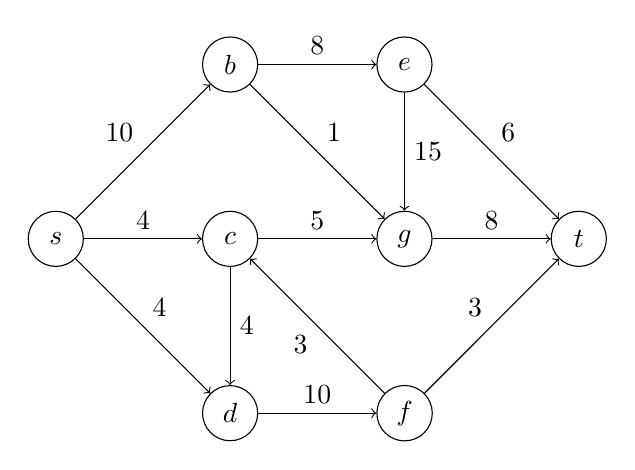
\begin{tikzpicture}
		[vertex/.style={circle, draw=black, node distance=1.5cm, minimum size=0.7cm}]
		\node[vertex] (s) {\(s\)};
		\node[vertex, right=of s] (c) {\(c\)};
		\node[vertex, above=of c] (b) {\(b\)};
		\node[vertex, below=of c] (d) {\(d\)};
		\node[vertex, right=of b] (e) {\(e\)};
		\node[vertex, right=of d] (f) {\(f\)};
		\node[vertex, right=of c] (g) {\(g\)};
		\node[vertex, right=of g] (t) {\(t\)};

		\draw[->] (s) to["10"] (b);
		\draw[->] (s) to["4"] (c);
		\draw[->] (s) to["4"] (d);
		\draw[->] (c) to["4"] (d);
		\draw[->] (b) to["8"] (e);
		\draw[->] (b) to["1"] (g);
		\draw[->] (e) to["15"] (g);
		\draw[->] (c) to["5"] (g);
		\draw[->] (d) to["10"] (f);
		\draw[->] (f) to["3"] (c);
		\draw[->] (f) to["3"] (t);
		\draw[->] (g) to["8"] (t);
		\draw[->] (e) to["6"] (t);
	\end{tikzpicture}
	\caption{A network}
	\label{q1}
\end{figure}

The first augmenting path which the algorithm finds can be \((s, b, e, t)\) (it may vary depending on the order that neighbours are selected in the BFS), through which a flow of 6 can be sent. The states of the graph at each point are shown in figure \ref{q1-steps}. (Saturated edges are omitted, and only remaining capacity is shown on each edge.)

The next augmenting path could be \((s, b, g, t)\) with a flow of 1. After this one, another possible augmenting path is \((a, c, g, t)\), which has a flow of 4. Next is \((s, d, f, t)\) with a flow of 3. The next augmenting path is \(s, b, e, g, t\). A flow of 2 can be sent through this one. The final augmenting path has a flow of 1, and is \((s, d, f, c, g, t)\).

Once there are no more augmenting paths to be found, we can sum up the flows through all the augmenting paths to find the maximal flow, which for this network is \(6 + 1 + 4 + 3 + 2 + 1 = 17\).

\begin{figure}[htbp]
	\centering
	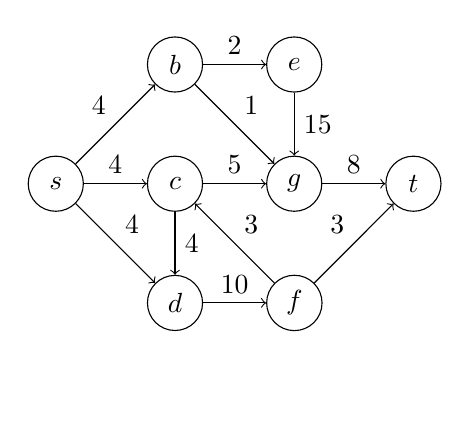
\begin{tikzpicture}
		[vertex/.style={circle, draw=black, node distance=0.8cm, minimum size=0.7cm, minimum size=0.7cm}]
		\node[vertex] (s) {\(s\)};
		\node[vertex, right=of s] (c) {\(c\)};
		\node[vertex, above=of c] (b) {\(b\)};
		\node[vertex, below=of c] (d) {\(d\)};
		\node[vertex, right=of b] (e) {\(e\)};
		\node[vertex, right=of d] (f) {\(f\)};
		\node[vertex, right=of c] (g) {\(g\)};
		\node[vertex, right=of g] (t) {\(t\)};
		\node[below=0.6cm of d]{};

		\draw[->] (s) to["4"] (b);
		\draw[->] (s) to["4"] (c);
		\draw[->] (s) to["4"] (d);
		\draw[->] (c) to["4"] (d);
		\draw[->] (b) to["2"] (e);
		\draw[->] (b) to["1"] (g);
		\draw[->] (e) to["15"] (g);
		\draw[->] (c) to["5"] (g);
		\draw[->] (d) to["10"] (f);
		\draw[->] (f) to["3" above right] (c);
		\draw[->] (f) to["3"] (t);
		\draw[->] (g) to["8"] (t);
	\end{tikzpicture}
	\hfill
	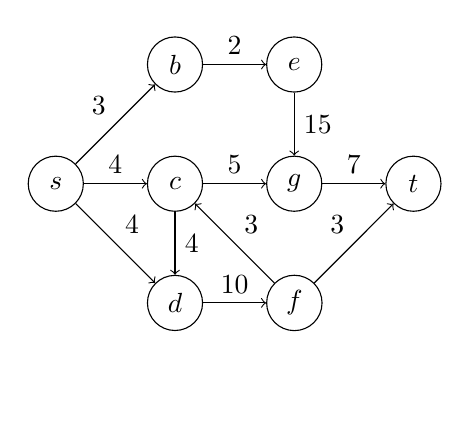
\begin{tikzpicture}
		[vertex/.style={circle, draw=black, node distance=0.8cm, minimum size=0.7cm}]
		\node[vertex] (s) {\(s\)};
		\node[vertex, right=of s] (c) {\(c\)};
		\node[vertex, above=of c] (b) {\(b\)};
		\node[vertex, below=of c] (d) {\(d\)};
		\node[vertex, right=of b] (e) {\(e\)};
		\node[vertex, right=of d] (f) {\(f\)};
		\node[vertex, right=of c] (g) {\(g\)};
		\node[vertex, right=of g] (t) {\(t\)};
		\node[below=0.6cm of d]{};

		\draw[->] (s) to["3"] (b);
		\draw[->] (s) to["4"] (c);
		\draw[->] (s) to["4"] (d);
		\draw[->] (c) to["4"] (d);
		\draw[->] (b) to["2"] (e);
		\draw[->] (e) to["15"] (g);
		\draw[->] (c) to["5"] (g);
		\draw[->] (d) to["10"] (f);
		\draw[->] (f) to["3" above right] (c);
		\draw[->] (f) to["3"] (t);
		\draw[->] (g) to["7"] (t);
	\end{tikzpicture}

	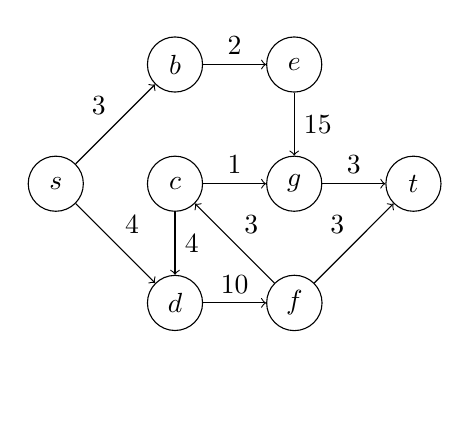
\begin{tikzpicture}
		[vertex/.style={circle, draw=black, node distance=0.8cm, minimum size=0.7cm}]
		\node[vertex] (s) {\(s\)};
		\node[vertex, right=of s] (c) {\(c\)};
		\node[vertex, above=of c] (b) {\(b\)};
		\node[vertex, below=of c] (d) {\(d\)};
		\node[vertex, right=of b] (e) {\(e\)};
		\node[vertex, right=of d] (f) {\(f\)};
		\node[vertex, right=of c] (g) {\(g\)};
		\node[vertex, right=of g] (t) {\(t\)};
		\node[below=0.6cm of d]{};

		\draw[->] (s) to["3"] (b);
		\draw[->] (s) to["4"] (d);
		\draw[->] (c) to["4"] (d);
		\draw[->] (b) to["2"] (e);
		\draw[->] (e) to["15"] (g);
		\draw[->] (c) to["1"] (g);
		\draw[->] (d) to["10"] (f);
		\draw[->] (f) to["3" above right] (c);
		\draw[->] (f) to["3"] (t);
		\draw[->] (g) to["3"] (t);
	\end{tikzpicture}
	\hfill
	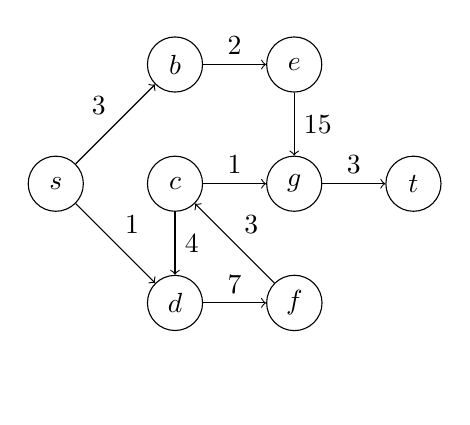
\begin{tikzpicture}
		[vertex/.style={circle, draw=black, node distance=0.8cm, minimum size=0.7cm}]
		\node[vertex] (s) {\(s\)};
		\node[vertex, right=of s] (c) {\(c\)};
		\node[vertex, above=of c] (b) {\(b\)};
		\node[vertex, below=of c] (d) {\(d\)};
		\node[vertex, right=of b] (e) {\(e\)};
		\node[vertex, right=of d] (f) {\(f\)};
		\node[vertex, right=of c] (g) {\(g\)};
		\node[vertex, right=of g] (t) {\(t\)};
		\node[below=0.6cm of d]{};

		\draw[->] (s) to["3"] (b);
		\draw[->] (s) to["1"] (d);
		\draw[->] (c) to["4"] (d);
		\draw[->] (b) to["2"] (e);
		\draw[->] (e) to["15"] (g);
		\draw[->] (c) to["1"] (g);
		\draw[->] (d) to["7"] (f);
		\draw[->] (f) to["3" above right] (c);
		\draw[->] (g) to["3"] (t);
	\end{tikzpicture}

	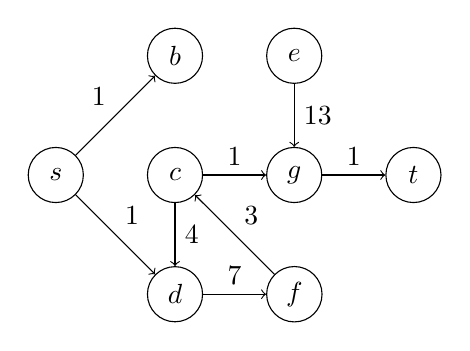
\begin{tikzpicture}
		[vertex/.style={circle, draw=black, node distance=0.8cm, minimum size=0.7cm}]
		\node[vertex] (s) {\(s\)};
		\node[vertex, right=of s] (c) {\(c\)};
		\node[vertex, above=of c] (b) {\(b\)};
		\node[vertex, below=of c] (d) {\(d\)};
		\node[vertex, right=of b] (e) {\(e\)};
		\node[vertex, right=of d] (f) {\(f\)};
		\node[vertex, right=of c] (g) {\(g\)};
		\node[vertex, right=of g] (t) {\(t\)};

		\draw[->] (s) to["1"] (b);
		\draw[->] (s) to["1"] (d);
		\draw[->] (c) to["4"] (d);
		\draw[->] (e) to["13"] (g);
		\draw[->] (c) to["1"] (g);
		\draw[->] (d) to["7"] (f);
		\draw[->] (f) to["3" above right] (c);
		\draw[->] (g) to["1"] (t);
	\end{tikzpicture}
	\hfill
	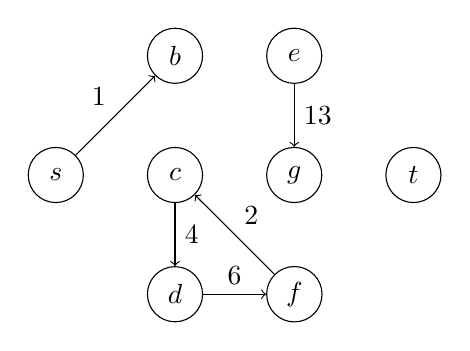
\begin{tikzpicture}
		[vertex/.style={circle, draw=black, node distance=0.8cm, minimum size=0.7cm}]
		\node[vertex] (s) {\(s\)};
		\node[vertex, right=of s] (c) {\(c\)};
		\node[vertex, above=of c] (b) {\(b\)};
		\node[vertex, below=of c] (d) {\(d\)};
		\node[vertex, right=of b] (e) {\(e\)};
		\node[vertex, right=of d] (f) {\(f\)};
		\node[vertex, right=of c] (g) {\(g\)};
		\node[vertex, right=of g] (t) {\(t\)};

		\draw[->] (s) to["1"] (b);
		\draw[->] (c) to["4"] (d);
		\draw[->] (e) to["13"] (g);
		\draw[->] (d) to["6"] (f);
		\draw[->] (f) to["2" above right] (c);
	\end{tikzpicture}
	\caption{The stages of the graph after sending sending flow through each shortest path}
	\label{q1-steps}
\end{figure}

\subsection*{Part B}

The minimal cut in the network must be a cut such that the sum of the capacities of the forward facing edges is minimal. We know however, that the capacity of the minimal cut must always be the same as the maximal flow. Therefore a minimal cut of the network in figure \ref{q1} must have a capacity of 17. One such cut is the following one.
\begin{equation*}
	(\{s, b\}, \{c, d, e, f, g, t\})
\end{equation*}

\end{document}